\section{Audit Decisions, Recovery, and Strong Baselines}
\label{sec:recovery-results}

\subsection{RQ3: What Does ICBA Authorize?}
Direct unshifted reuse fails every candidate certificate in the original refresh replay and routes all 20 targets to the endpoint. ICBA therefore blocks unsafe efficiency without manufacturing a saving. TCP changes the candidate before certification. The original allocation accepts 19/20 candidates; the $.025+.025$ sensitivity accepts all ten SIFT and six Arxiv candidates, with four certified endpoint fallbacks and no abstention.

\begin{figure*}[t]
\centering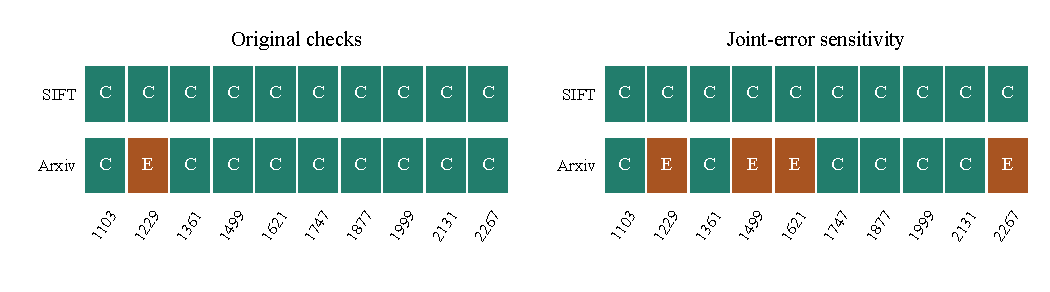
\includegraphics[width=\textwidth]{figures/decisions.pdf}
\caption{Completed target decisions. C denotes candidate and E endpoint fallback. The stricter $.025+.025$ allocation changes Arxiv composition from nine to six candidates while every completed decision remains qualified.}
\label{fig:decisions}
\Description{SIFT accepts ten candidates under both rules. Arxiv accepts nine under the original allocation and six under the stricter allocation.}
\end{figure*}

\subsection{RQ4: Endpoint-Relative Recovery and Incremental Value}
TCP's original completed decisions reduce mean NDC by 44.39\% on SIFT and 44.79\% on Arxiv. Under the joint-error allocation, SIFT is unchanged and Arxiv retains 29.86 [14.75,45.00]\%. Risk is 1.79\% and 1.68\%, respectively. Both remain positive relative to each target's endpoint.

The equal-information comparison asks the stronger question. Against target-global calibration with the same 500 selection, 500 certification, and 1,000 evaluation queries, TCP gains a further 27.60 [17.92,36.72]\% mean NDC on SIFT, but Arxiv's 10.78\% interval includes zero and its p95 ratio is 1.109. Query conditioning therefore adds resolved value only on SIFT under the registered event, grid, and SLA.

\begin{figure}[t]
\centering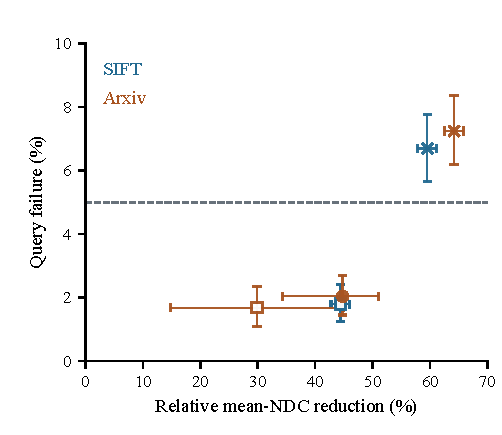
\includegraphics[width=\linewidth]{figures/tradeoff.pdf}
\caption{Refresh risk--work tradeoff with crossed 95\% intervals. Direct reuse is efficient but crosses the risk target; certification and fallback move completed decisions toward the endpoint.}
\label{fig:tradeoff}
\Description{Direct reuse has high failure. Target-recalibrated policies have lower risk and retain positive search-work savings.}
\end{figure}

\subsection{Prospective Fresh-Build Confirmation}
\label{sec:prospective}
\label{sec:fresh-bridge}
S9-3 freezes a one-rung candidate before eight new insertion-permutation builds and three fresh query roles per dataset are accessed. All 56 directed decisions per dataset accept the candidate, with zero fallback or abstention (Table~\ref{tab:s9-prospective}). Across 144,000 response cells and 112,000 raw timing measurements, native and measured top-$k$ agree exactly. Sparse-grid and 2.5\%-risk sensitivities remain safe but collapse to the endpoint, defining preregistered boundaries rather than failures of the primary configuration.

\begin{table*}[t]
\caption{S9-3 prospective confirmation on eight new target builds per dataset. Risk and wall-time reduction are percentages [95\% crossed target-build/query interval]. P95 is the policy/endpoint wall-time ratio [95\% interval]; LOTO is minimum wall-time reduction after deleting one target.}
\label{tab:s9-prospective}
\small\begin{tabular*}{\textwidth}{@{\extracolsep{\fill}}lrrrr@{}}\toprule
Dataset & Eval. risk & Wall-time reduction & P95 ratio & LOTO reduction\\\midrule
\SProspectiveRows
\bottomrule\end{tabular*}
\end{table*}

\subsection{Strong Baselines Change the Method Conclusion}
S9-4 evaluates fixed and target-calibrated policies on the same prospective indexes with new disjoint roles (Table~\ref{tab:s9-baselines}). Every deployable arm passes risk, mean-wall, p95, LOTO, and timing-stability gates. Fixed-256 exactly matches source one-rung on SIFT and exceeds it by 10.91 wall-time percentage points on Arxiv. The source heuristic is therefore unnecessary on this panel.

The equal-information target-global-500 arm remains safe and positive but falls back on 7/56 decisions per dataset, widening its interval. With 500 selection plus 500 certification labels, target-global-1000 is strongest on both datasets. This is a label-value result, not an equal-information victory. The evaluation oracle leaves additional SIFT headroom; on Arxiv, the label-rich target arm reaches the oracle action pattern.

\begin{table*}[t]
\caption{S9-4 paired strong-baseline audit. Risk and wall-time reduction are percentages [95\% crossed interval]. P95 gives ratio (95\% upper bound); LOTO is minimum reduction. Target-global-500 uses 500 labels total, target-global-1000 uses 1,000.}
\label{tab:s9-baselines}
\small\begin{tabular*}{\textwidth}{@{\extracolsep{\fill}}llrrrr@{}}\toprule
Dataset & Candidate & Risk & Wall-time reduction & P95 ratio & LOTO\\\midrule
\SStrongBaselineRows
\bottomrule\end{tabular*}
\end{table*}

\paragraph{Mechanism attribution.}
Moving one rung above the source action lowers held-out risk from 2.15\% to 0.40\% on SIFT and from 1.775\% to 0.307\% on Arxiv, while sacrificing 24.92 and 31.21 NDC-gain points. Certification changes authorization but not execution when every candidate passes. Target labels, rather than source-specific tailoring, drive the largest additional gains.

\subsection{RQ5--RQ6: Tail and Build Stability}
For historical joint-error TCP, pooled p95/p99 remain below the endpoint and every target has non-increasing tails. S9-3 and S9-4 also pass p95 and LOTO gates; the least favorable S9-4 p95 upper bound is 0.930 for SIFT target-global-500 and 0.921 for its Arxiv counterpart. The prospective conclusions therefore do not depend on one target build, although eight builds remain an underpowered basis for open-population inference.
